\documentclass{article}%
\usepackage[T1]{fontenc}%
\usepackage[utf8]{inputenc}%
\usepackage{lmodern}%
\usepackage{textcomp}%
\usepackage{lastpage}%
\usepackage{authblk}%
\usepackage{graphicx}%
%
\title{Identification of the pollen self{-}incompatibility determinant in Papaver rhoeas}%
\author{Kathleen Arellano}%
\affil{Department of Bioengineering, University of California, Berkeley, California 94720, USA}%
\date{01{-}01{-}2010}%
%
\begin{document}%
\normalsize%
\maketitle%
\section{Abstract}%
\label{sec:Abstract}%
Researchers at the Weill Cornell Medical College have discovered a new therapeutic component of tumor suppression, stimulating the production of monocytes (which kill cancer cells) from specialized skin cells derived from human leukocytes.\newline%
They developed a class of mesenchymal{-}derived skin cells that have approximately two{-}thirds of the specificity needed for tumor growth. This specificity means that these skin cells can then be infused into organs such as the lungs, liver, and potentially various organs.\newline%
One unique feature of the mesenchymal skin cells is their interleukin{-}1 (IL{-}1) transfer rate, which is exponentially higher than natural skin cells because they are non{-}derived skin cells. In fact, though the amount of IL{-}1 in each skin cell is regulated according to the patients overall health, the higher availability of IL{-}1 is believed to suppress tumor growth.\newline%
IL{-}1 is known to play a central role in killing tumor cells, as well as to aid the growth of cancer stem cells or lines that line a tumor. Immunosuppressant drugs rely on IL{-}1 to help tumors resist apoptosis and eliminate disease cells, but scientists still dont fully understand what happens at the cellular level when such molecules are present.\newline%
In their analysis of the skin cells results, the researchers found that the presence of IL{-}1 activates the differentiation factor{-}Caspase{-}1 (iC.C.P.). The activation of iC.C.P. facilitates tumor growth in vitro and also empowers tumor suppressor cells like the skin cells to regulate their own internal growth.\newline%
Because it lacks a visible characteristic, skin cells derived from cloned skin cells were not allowed to differentiate into skin cells. However, they were able to recognize the skin cells small fluorescent marker and allow a rapid transition between cells.\newline%
Himanshu Sanghavi, assistant professor of medicine at Weill Cornell Medical College, and lead author of the paper, is a nationally recognized expert in skin biology.\newline%
Using skin cells derived from tumor{-}derived skin cells will enable medical researchers to more specifically discover who the winners are in this very competitive field, said Sanghavi. It is also important to know who the losers are; those who have the most difficulty producing IL{-}1, among other characteristics, are the ones that may benefit the most from thiopental chemotherapy.\newline%
The study was published in the journal Molecular Therapy.

%
\subsection{Image Analysis}%
\label{subsec:ImageAnalysis}%


\begin{figure}[h!]%
\centering%
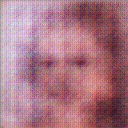
\includegraphics[width=150px]{500_fake_images/samples_5_35.png}%
\caption{A Close Up Of A Black And White Cat}%
\end{figure}

%
\end{document}